\setchapterpreamble[u]{\margintoc}
\chapter{Diagramma di stato Fe-C}\label{Fe-C}
\labch{cap8}

Il ferro puro presenta due diverse forme allotropiche:
\begin{itemize}
    \item configurazione CCC a 907°C;
    \item CFC da 907°C a 1394°C;
    \item CCC fino alla temperatura di fusione di 1537°C.
\end{itemize}

In presenza di \textbf{carbonio}, che è un elemento austenitizzante, cioè un elemento che stabilizza la fase austenitica e ne ampia l’esistenza, le forme allotropiche cambiano e si originano diverse \textbf{soluzioni solide}. Si ha:
\begin{itemize}
    \item \textbf{ferrite} \mathtext{\boldsymbol\alpha}, in cui la solubilità di carbonio è 0,02-0,03\% a 723°C nella configurazione CCC;
    \item \textbf{austenite} \mathtext{\boldsymbol\gamma},  in cui il tenore di carbonio è del 1,98-2\% a 1130 °C (1135 °C) nella configurazione CFC;
    \item \textbf{ferrite} \mathtext{\boldsymbol\delta}, n cui la solubilità massima del carbonio è dello 0,1\% a 1492°C configurazione CCC. La maggior solubilità del carbonio nell’ultima configurazione rispetto alla ferrite \mathtext{\alpha} deriva dalle dilatazioni termiche.
\end{itemize}

L'aggiunta di elementi leganti può portare ad un aumento o ad una diminuzione del campo austenitico. Sono elementi austenitizzanti (ovvero che aumentano il campo di esistenza del ferro $\gamma$) il carbonio, il nichel, il manganese, l'azoto. Il cromo è invece un elemento ferritizzante (aumenta il campo di esistenza del ferro $\alpha$ e $\delta$.)

\begin{figure}[h]
\centering
    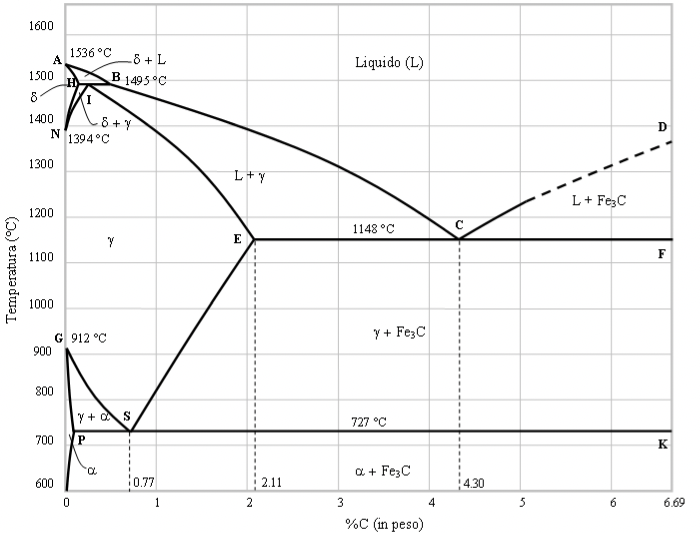
\includegraphics[width=1\textwidth]{images/img31.png}
    \caption{Diagramma Fe-C per percentuali di C inferiori al 6,69\% (cementite)}
    \labfig{img31}
\end{figure}
\index{peritettico}
\textbf{PERITETTICO (punto I): Liquido (0,18 \%C) + ferro \mathtext{\boldsymbol\delta} (0,1 \%C)→ austenite \mathtext{\boldsymbol\gamma} (0,5 \%C)}\\
La trasformazione peritettica avviene a 1492 °C con tenore di carbonio pari allo 0,18\%. Nel peritettico vi è la trasformazione di una fase solida, cioè l’austenite, sottoposta a riscaldamento, in una fase liquida e una solida, cioè la ferrite \mathtext{\delta}.\\
Il punto peritettico è importante nei fenomeni di solidificazione.\\
Esso infatti da origine a due fenomeni.\\
Si può avere il \textbf{salto del peritettico}, se la trasformazione non avviene in condizioni di equilibrio, cioè non avendo la presenza di un liquido con 0,5\% di carbonio e un solido con tenore 0,1\% di C. Si ha una zona stratificata con bande di liquido e solido, con la parte liquida più all’interno in quanto solidifica più lentamente. Tale fenomeno prende il nome di \textbf{bandizzazione} o \textbf{stratificazione}.
L’altro fenomeno è la \textbf{differente cristallografia e morfologia} tra superficie e cuore del lingotto. In superficie si originano dei cristalli molto piccoli e fini perché siamo in presenza di elevata nucleazione di cristalli; nelle zone sotto la superficie i cristalli si allungano dando vita a una struttura dendritica a palizzata; infine nel cuore vi è una struttura poligonale. Ci si può trovare davanti, quindi, ad un materiale che è chimicamente e cristallograficamente disomogeneo.\\
A questo problema si può ovviare tramite la \textbf{ricottura}, in modo da omogeneizzare completamente la struttura, e tale processo prevede un riscaldamento del lingotto fino alla temperatura più alta possibile (a circa 1200°C) e successivo raffreddamento lento. In realtà la ricottura avviene solo per acciai di altissimo pregio: infatti, le colate non avvengono più in lingotteria, da cui si originano i lingotti, ma si preferisce utilizzare la \textbf{colata in continua}, in cui la solidificazione avviene simultaneamente alla prima laminazione. Non appena si forma una pellicola di solido sufficientemente spessa e tale da resistere ad azioni meccaniche, si comincia a laminare. Il prodotto in uscita dalla colata in continua si chiama \textbf{bramma}, cioè il grezzo di colata che ha già subito la prima laminazione. Non si ha in tal modo la struttura a palizzata e si sfrutta il calore del materiale che sta solidificando e che cede calore all’aria.

\index{eutettico}
\textbf{EUTETTICO (punto C): Liquido (4,30 \%C) → austenite + cementite \mathtext{Fe_3C} o grafite}\\
La trasformazione eutettica avviene a \textbf{1130°C} con tenore di carbonio pari al 4,3\%: si ha del liquido che, solidificando (raffreddamento), si trasforma in austenite più una fase che a seconda delle condizioni può essere o grafite o cementite.\\
Se il raffreddamento è lento e non vi sono elementi grafitizzanti, allora la trasformazione eutettica porta alla formazione di austenite e cementite. Se, invece, il raffreddamento è comunque lento, ma sono presenti elementi grafitizzante, allora si forma la grafite.\\
Qualora la seconda fase sia la cementite, la miscela formata da austenite e cementite è chiamata \textbf{ledeburite}.

\index{acciaio}
Se si supera il punto E, con \%C pari a 2,2\%, si entra nel campo delle \textbf{ghise}. Se la \%C è inferiore al 2\%, cioè siamo nel campo degli \textbf{acciai}, essi non sono interessati alla trasformazione eutettica, cioè nella solidificazione non è presente l’eutettico. Tuttavia esistono acciai speciali con \%C > 2, cioè gli acciai refrattari, e anche ghisa con \%C < 2.

Le ghise sono dei materiali la cui caratteristica principale è la colabilità, sono cioè \textbf{leghe da getto}. Con le ghisa, si cerca di ottenere il manufatto il più possibile simile al risultato finale a ridosso della solidificazione, per ridurre il più possibile le lavorazioni successive.\\
Il requisito per una \textbf{facile colabilità} è quello di avere una temperatura di colata e di solidificazione più basse possibili, temperature che corrispondono a quella del punto eutettico, che è il punto nel quale vi è liquido alla temperatura più bassa possibile. In questo punto si passa da un 100\% di liquido a 100\% di solido, mentre in tutti gli altri punti si ha la coesistenza di liquido e solido: quindi nel punto eutettico non si ha un intervallo di solidificazione. Attraverso la colata, si posso realizzare pezzi dalla forma complessa.\\
Se si ha la coesistenza di liquido e solido ci si trova in presenza di un \textbf{fango}, che ha elevata viscosità, con il rischio che esso non riempia bene lo stampo, ottenendo di conseguenza dei getti difettosi. Quindi tutte le volte che si ha un materiale da getto (ghisa, ottone, bronzo, leghe d’allumunio) la \textbf{composizione} deve essere quella \textbf{più vicina possibile a quella dell’eutettico}. Infatti, maggiore è l’intervallo di solidificazione, maggiori sono le probabilità di avere fanghi e di conseguenza, stampi difettosi.

In realtà, se si colasse una ghisa con tenore di carbonio 4,3\% (cioè quella che esce dall’altoforno), essa sarebbe troppo fragile, con modestissime caratteristiche meccaniche.
Utilizzando, però, un tenore di carbonio inferiore, quindi muovendosi verso sinistra nel diagramma di stato, si avrebbe la solidificazione dell’austenite, con formazione di cristalli austenitici, e il carbonio si andrebbe a posizionare a bordo di grano, infragilendo ulteriormente il materiale.
La soluzione di questo problema si ha aggiungendo un terzo elemento, cioè il \textbf{silicio}\index{silicio}. Si ottengono, così, le ghise al ferro-carbonio-silicio.\\
Questo elemento aumenta l’attività del carbonio, cioè, in presenza di silicio, il carbonio diventa più attivo e si comporta come se ce ne fosse di più della sua reale quantità. Il silicio è un \textbf{attivizzante di carbonio C}. L’effetto energizzante è di 1:3, cioè 3 parti di silicio fanno si che il carbonio si comporti come se ce ne fosse una parte in più (0,3\% Si \mathtext{\to} + 0,1\% di C). Mettendo il 3\% del silicio, e calcolando il carbonio equivalente si arriva a un tenore di carbonio che è 4,3\%, quando nella realtà il carbonio effettivamente presente è circa del 3\%. Tale tenore di carbonio è accettabile dal punto di vista meccanico.

Un’altra tecnica utilizzata in questo ambito, oltre alla modifica della composizione chimica, è la cosiddetta \textbf{inoculazione}, che serve ad avere grafite che, sotto forma di lamelle, è uniformemente distribuita nella ghisa, che è chiamata in questo caso \textbf{ghisa lamellare}. L’inoculazione consiste nell’aggiungere al momento della colata un ulteriore 0,1\% di silicio sotto forma di polvere, in modo uniforme sul bagno liquido di ghisa che sta solidificando: localmente il silicio aumenta di molto l’attività di carbonio, arrivando in condizioni ipereutettiche, perché vi è l’attività energizzante del silicio. In queste condizioni, la prima fase a solidificare è la grafite, che non andrà a posizionarsi a bordo grano, ma è distribuita uniformemente su una matrice che segue il diagramma di stato Fe-C. La ghisa ha la forma di dischetto, ma in sezione ha la forma di lamella.\\
Gestendo bene l’operazione, si riesce a ottenere una distribuzione uniforme della grafite su una \textbf{matrice perlitica} (raffreddando una lega al 2\% ci carbonio) oppure, raffreddando molto lentamente, su una \textbf{matrice ferritica}.\\
La lamella di ghisa ha gli apici aguzzi con fattore di intaglio pari a 13. Ciò significa che agli apici della lamella, gli sforzi sono intensificati di un fattore pari a 13.

Una variante a questo tipo di ghisa è la \textbf{ghisa sferoidale}, dove la grafite al posto di essere in forma lamellare è in forma sferoidale. Essa presenta il vantaggio di avere un fattore di intaglio pari a 3, cioè permette di avere un materiale a basso costo con caratteristiche meccaniche più elevate e paragonabili agli acciai. Infatti, gli acciai da bonifica sono molto costosi.
La forma sferica si ottiene aggiungendo dopo l’inoculazione un ulteriore 0,1\% di \textbf{magnesio Ma}\index{magnesio}, che ha lo scopo di alterare la tensione superficiale della grafite in fase di solidificazione. La grafite così solidifica a forma sfeiroidale.\\
In questo caso è previsto un allungamento, a differenza della ghisa lamellare.

Combinando l’\textbf{aggiunta di silicio} ad un \textbf{raffreddamento lento}, si ha un’elevata \textbf{grafitizzazione}.

Se, invece, si \textbf{raffredda velocemente} con la presenza di una \textbf{bassa percentuale di silicio}, durante la trasformazione eutettica, si inibisce la formazione di grafite a favore della cementite, ottenendo le cosiddette \textbf{ghise bianche}, formate da placche di cementite.\\
Essendo la cementite una fase dura e caratterizzata da grandi cristalli bianchi, si aggiungono elementi leganti del carbonio che favoriscono la formazione dei propri carburi (vanadio, niobio) e si ottiene un materiale molto duro e poco costoso.

Tuttavia, si tende ad espellere carbonio e formare grafite.

Una via di mezzo è la \textbf{ghisa trotata}, dove si ha coesistenza di grafite e cementite, cioè il carbonio è solidificato in entrambe le forme. Tale ghisa però è uno scarto in quanto non è utile.

Nelle ghise si può avere il cosiddetto \textbf{occhio di bue}: ad esempio, nella ghisa sferoidale si ha un cerchio nero di grafite sferoidale, che contiene la maggior parte di carbonio, circondato dalla ferrite che è bianca e priva di carbonio.

\index{eutettoidico}
\textbf{PUNTO EUTETTOIDICO (punto S): Austenite \mathtext{\boldsymbol\gamma \to} ferrite \mathtext{\boldsymbol\alpha} (0,02 \%C) + cementite \mathtext{\boldsymbol{Fe_3C}} (6,66 \%C)}\\
La trasformazione eutettoidica si trova a una temperatura di \textbf{723°C} con tenore di carbonio pari allo 0,8\%. In questo punto si ha una fase solida di alta temperatura, cioè l’austenite, che al raffreddamento genera due fasi solide di differente composizione (ferrite allo 0,02\% di C e cementite al 6,66\% di C).\\
Se ci si trova proprio del \mathtext{punto eutettoidico}, la miscela meccanica che solidifica con 89\% di ferrite e 11\% di cementite è chiamata \textbf{perlite}.\\ \index{perlite}
Se \textbf{\%C < 0,8}, la ferrite \mathtext{\alpha} solidifica prima, cioè si trasforma precedentemente a causa del raffreddamento dell’austenite: quindi, si ha \textbf{ferrite e perlite}.\\
Se \textbf{\%C > 0,8}, si ha \textbf{cementite e perlite}. La trasformazione eutettoidica è:
\begin{equation*}
    \gamma(0,8\%\mathtext{C})\to\alpha(\simeq0\%\mathtext{C})+\mathtext{Fe_3C(6,66\%)}
\end{equation*}
La ferrite \mathtext{\alpha} non contiene carbonio, che invece è interamente contenuto nella cementite.

Tale trasformazione è governata dai \textbf{meccanismi di diffusione}, che a sua volta dipende dalla temperatura e dal tempo (legge di Fick), oltre che dalla forza spingente (che in questo caso è la differenza di concentrazione); l’effetto predominante è quello della temperatura perché di tipo esponenziale (\mathtext{e^{1/T}}), mentre l’effetto del tempo è sotto radice quadrata (\mathtext{t^{1/2}}).\\
Questa trasformazione avviene attraverso processi di \textbf{nucleazione}, che consiste nella formazione nuclei di ferrite e cementite, quindi creando una  \textbf{struttura lamellare}, perché la ferrite è priva di carbonio, che invece è totalmente contenuto nella cementite. Il processo successivo è la \textbf{crescita dei nuclei} con il tempo.